% ModPINN architecture: original TikZ adaptation of the article's Figure 2.
\documentclass[tikz,border=6pt]{standalone}
\usepackage[T1]{fontenc}
\usepackage{amsmath,amssymb,mathptmx}
\usetikzlibrary{arrows.meta,calc,positioning,backgrounds}
\ifdefined\darkmode
  \definecolor{ink}{HTML}{E6EDF3}
  \definecolor{muted}{HTML}{A4B1C1}
  \definecolor{panel}{HTML}{151D29}
  \definecolor{feature}{HTML}{302637}
  \definecolor{featureline}{HTML}{D4A4BC}
  \definecolor{network}{HTML}{21374C}
  \definecolor{networkline}{HTML}{77BDE8}
  \definecolor{physical}{HTML}{203A33}
  \definecolor{physicalline}{HTML}{77C7AC}
\else
  \definecolor{ink}{HTML}{242C38}
  \definecolor{muted}{HTML}{596778}
  \definecolor{panel}{HTML}{FAF6F8}
  \definecolor{feature}{HTML}{F5E1E8}
  \definecolor{featureline}{HTML}{9B6179}
  \definecolor{network}{HTML}{E0EDF8}
  \definecolor{networkline}{HTML}{326C96}
  \definecolor{physical}{HTML}{E3F1EB}
  \definecolor{physicalline}{HTML}{397F66}
\fi
\begin{document}
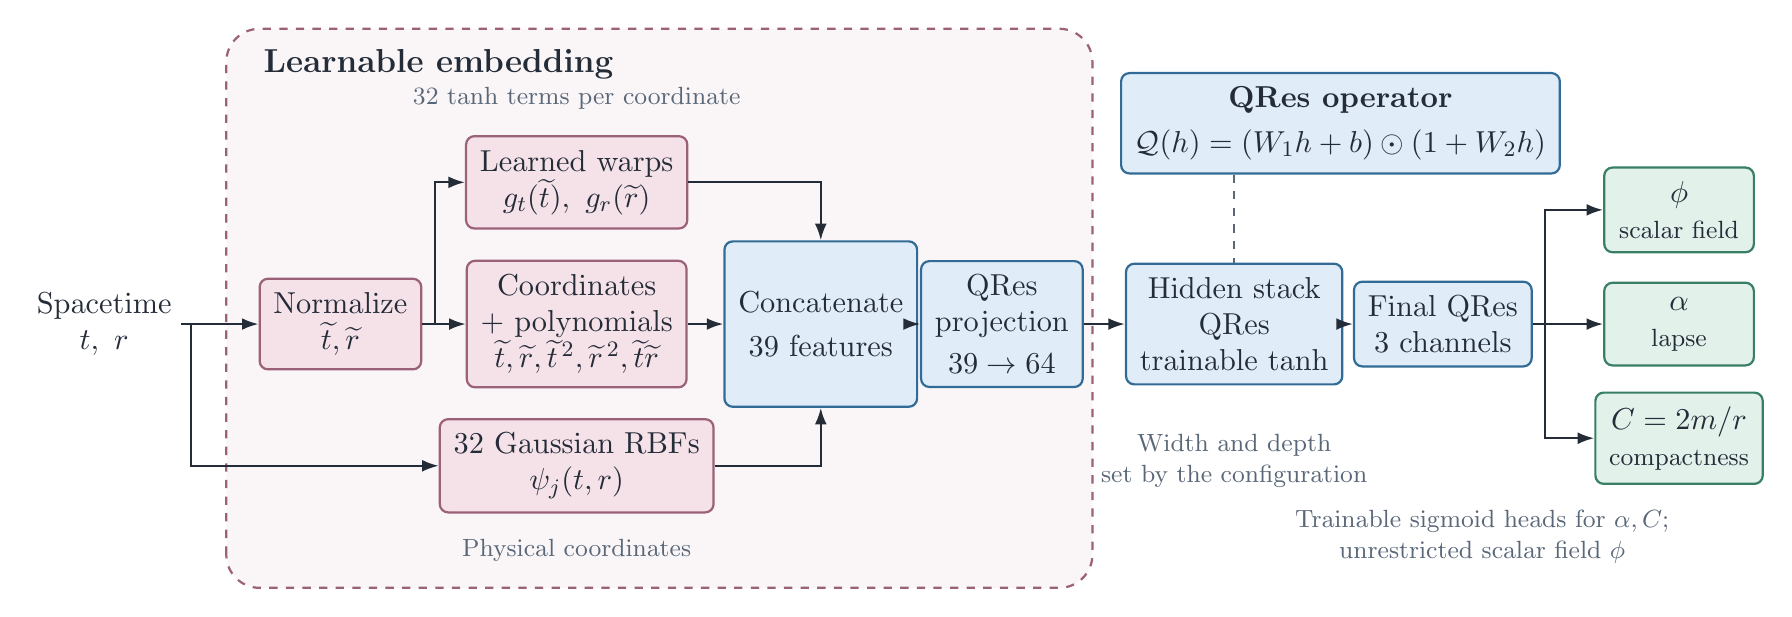
\begin{tikzpicture}[
  font=\fontsize{11}{13}\selectfont, text=ink,
  flow/.style={-{Latex[length=2.1mm,width=1.5mm]},draw=ink,line width=.8pt},
  link/.style={draw=ink,line width=.8pt},
  block/.style={rounded corners=3pt,draw=featureline,fill=feature,
    line width=.8pt,align=center,minimum height=1.05cm,inner sep=5pt},
  net/.style={block,draw=networkline,fill=network},
  fieldbox/.style={block,draw=physicalline,fill=physical,minimum width=1.9cm},
  small/.style={font=\fontsize{9.5}{11}\selectfont,text=muted,align=center}
]
% Main data path and the two independent coordinate branches.
\node[align=center] (input) at (0,0) {Spacetime\\$t,\ r$};
\coordinate (raw) at (1.1,0);
\node[block,minimum width=1.7cm] (norm) at (3.0,0) {Normalize\\$\widetilde t,\widetilde r$};
\coordinate (normalized) at (4.2,0);
\node[block,minimum width=2.4cm] (warp) at (6.0,1.8)
  {Learned warps\\$g_t(\widetilde t),\ g_r(\widetilde r)$};
\node[small,above=2mm of warp] {32 tanh terms per coordinate};
\node[block,minimum width=2.4cm] (poly) at (6.0,0)
  {Coordinates\\+ polynomials\\$\widetilde t,\widetilde r,\widetilde t^{\,2},\widetilde r^{\,2},\widetilde t\widetilde r$};
\node[block,minimum width=2.4cm] (rbf) at (6.0,-1.8)
  {32 Gaussian RBFs\\$\psi_j(t,r)$};
\node[small,below=2mm of rbf] {Physical coordinates};
\node[net,minimum width=1.6cm,minimum height=2.1cm] (concat) at (9.1,0)
  {Concatenate\\[3pt]39 features};
\node[net,minimum width=1.6cm] (projection) at (11.4,0)
  {QRes\\projection\\[2pt]$39\to64$};
\draw[link] (input.east) -- (raw);
\draw[flow] (raw) -- (norm.west);
\draw[flow] (raw) -- (raw |- rbf.west) -- (rbf.west);
\draw[link] (norm.east) -- (normalized);
\draw[flow] (normalized) -- (normalized |- warp.west) -- (warp.west);
\draw[flow] (normalized) -- (poly.west);
\draw[flow] (warp.east) -- (concat.north |- warp.east) -- (concat.north);
\draw[flow] (poly.east) -- (concat.west);
\draw[flow] (rbf.east) -- (concat.south |- rbf.east) -- (concat.south);
\draw[flow] (concat.east) -- (projection.west);
% Quadratic hidden stack and three output channels.
\node[net,minimum width=2.0cm,minimum height=1.35cm] (hidden) at (14.35,0)
  {Hidden stack\\QRes\\trainable tanh};
\node[net,minimum width=1.5cm] (final) at (17.0,0)
  {Final QRes\\3 channels};
\coordinate (split) at (18.3,0);
\node[fieldbox] (phi) at (20.0,1.45) {$\phi$\\\small scalar field};
\node[fieldbox] (alpha) at (20.0,0) {$\alpha$\\\small lapse};
\node[fieldbox] (compactness) at (20.0,-1.45) {$C=2m/r$\\\small compactness};
\draw[flow] (projection.east) -- (hidden.west);
\draw[flow] (hidden.east) -- (final.west);
\draw[link] (final.east) -- (split);
\draw[flow] (split) -- (split |- phi.west) -- (phi.west);
\draw[flow] (split) -- (alpha.west);
\draw[flow] (split) -- (split |- compactness.west) -- (compactness.west);
\node[small,below=5mm of hidden] {Width and depth\\set by the configuration};
\node[small] at (17.5,-2.7) {Trainable sigmoid heads for $\alpha,C$;\\unrestricted scalar field $\phi$};
% Operator callout, as in the paper, without obscuring the forward path.
\node[net,minimum width=5.4cm,minimum height=1.0cm] (operator) at (15.7,2.55)
  {\textbf{QRes operator}\\[3pt]
   $\mathcal Q(h)=(W_1h+b)\odot(1+W_2h)$};
\draw[draw=muted,dashed,line width=.7pt] (operator.south -| hidden.north) -- (hidden.north);
% The title lane stays above all embedded branches and labels.
\begin{scope}[on background layer]
  \draw[rounded corners=12pt,draw=featureline,fill=panel,dashed,line width=.8pt]
    (1.55,-3.35) rectangle (12.55,3.75);
\end{scope}
\node[anchor=west,font=\bfseries\fontsize{12}{14}\selectfont]
  at (1.9,3.3) {Learnable embedding};
\end{tikzpicture}
\end{document}
